
\section*{Exercises}
\addcontentsline{toc}{section}{Exercises}

\begin{excersizelist}

\item \label{exer:multiplieropampwithmodel}  Analyse the inverting amplifier circuit in Figure~\zref{circ:opampinvertingamplifierequivalent} to obtain the relationship between input voltage $x$ and output voltage $y$ given by~\zeqref{eq:intertingopampmodel}.  You may wish to use a symbolic programming language (for example Maxima, Sage, Mathematica, or Maple).
\begin{solution}
We provide two solutions.  Let $v_i$, $v_o$, $v_1$ and $v_2$ be the voltages over the input resistor $R_i$, the output resistor $R_o$, and resistors $R_1$ and $R_2$ respectively.  We have 8 unknown voltages $x,y,v_i,v_1,v_2,v_o,v_+,v_-$.  We will need 7 independent equations to find an equation relating $x$ and $y$.  All currents are considered to be flowing either downwards or to the right in the circuit diagram.  The first 4 equations are given by voltages over each resitor,
\begin{align*}
x &= v_- + v_1 \\
v_- &= y + v_2 \\
v_- &= v_+ + v_i \\
y &= v_o + A(v_+ - v_-) 
\end{align*}
The next two equations apply Kirchoff's current law to each node betweeen resistors.  The currents into the 3 way connection between $R_i, R_1$ and $R_2$ sum to zero, and so
\[
\frac{v_1}{R_1} = \frac{v_2}{R_2} + \frac{v_i}{R_i}
\]
by Ohm's law.  Finally the currents through $R_o$ and $R_2$ are the same, and so
\[
\frac{v_o}{R_o} = \frac{v_2}{R_2}.
\]
The final equation simply observes that the non-inverting terminal $v_+$ is connected to ground
\[
v_+ = 0.
\]
We now have 7 linearly independent equations for the 8 unknowns $x,y,v_i,v_1,v_2,v_o,v_+,v_-$.  We can use these to find an equation that describes $y$ in terms of $x$.  The Mathematica command
\begin{verbatim}
Simplify[Solve[{x == vm + v1,
   vm == y + v2,
   vm == vp + vi,
   y == vo + A*(vp - vm),
   v1/r1 == vi/ri + v2/r2,
   vo/ro == v2/r2,
   vp == 0,
   r1 > 0, r2 > 0, ro > 0, ri > 0, A > 0},
  {y,vi,vo,v2,v1,vp,vm}, Reals]]
\end{verbatim}
or Maxima command
\begin{verbatim}
linsolve([x=vm+v1,
          vm=y+v2,
          vm=vp+vi,
          y=vo+A(vp-vm),
          v1/R1=v2/R2+vi/Ri,
          v2/R2=vo/Ro,
          vp=0],
          [y,vp,vm,v1,v2,vo,vi]);
\end{verbatim}
readily obtains
\[
y = \frac{R_i (R_o - A R_2) }{R_i (R_2+R_o)+R_1 (R_2+R_i + A R_i+R_o)}x.
\]

The second solution is thanks to Badri Vellambi.  Badri sets $v_i = v_+ - v_-$ so that the voltage over the dependent voltage source is $Av_i$.  Consider the operational amplifier circuit with feedback presented in Fig.~\ref{Fig-Prob2.1a}. Suppose that the voltage signal fed into the circuit is $x(t)$ and the voltage signal measured at the output of the opamp is $y(t)$. 

{
\centering
\captionsetup{type=figure}
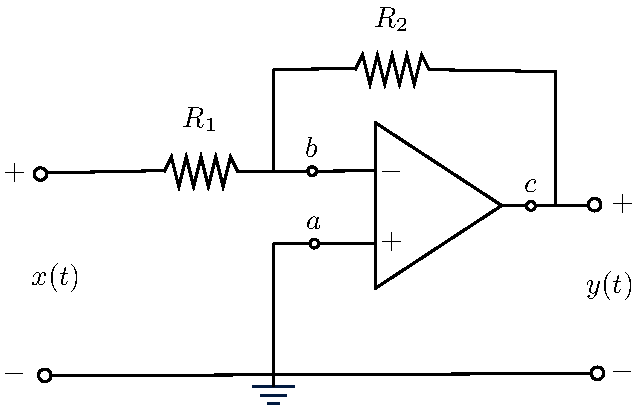
\includegraphics[width=3in]{plots/multiplierbadri1.pdf}
\captionof{figure}{The circuit}
 \label{Fig-Prob2.1a}
}

To simplify the circuit, one has to use the model for the opamp given in Fig.~\ref{Fig-Prob2.1b} which involves the voltage-controlled voltage-source (VCVS) at the output side (indicated in green).  While replacing the operational amplifier with its model, it must be noted that the positive terminal of the operational amplifier is connected to the ground.

{
\centering 
\captionsetup{type=figure}
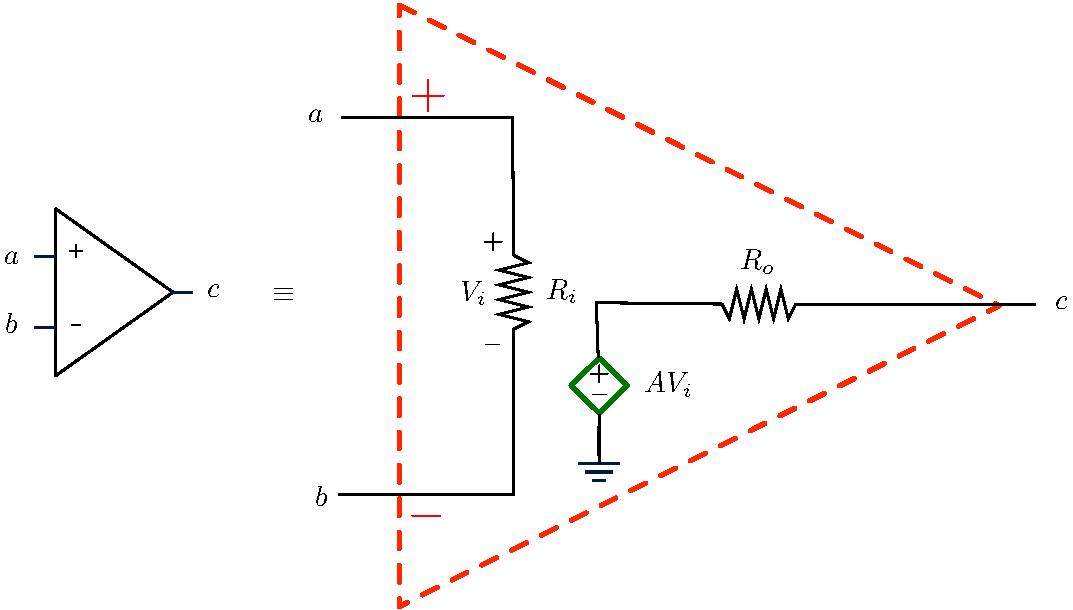
\includegraphics[width=5in]{plots/multiplierbadri2.pdf}
\captionof{figure}{The model for an operational amplifier}
 \label{Fig-Prob2.1b}
}

Upon replacement, we obtain the following equivalent circuit. Again notice that since the positive terminal of the opamp was connected to the ground, the voltage output by the VCVS is $AV_i$ where $V_i$ is the voltage between the ground and the top of the resistance $R_i$, and is measured against the flow of the current $i-i_1$ as is indicated in the figure.

{
\centering 
\captionsetup{type=figure}
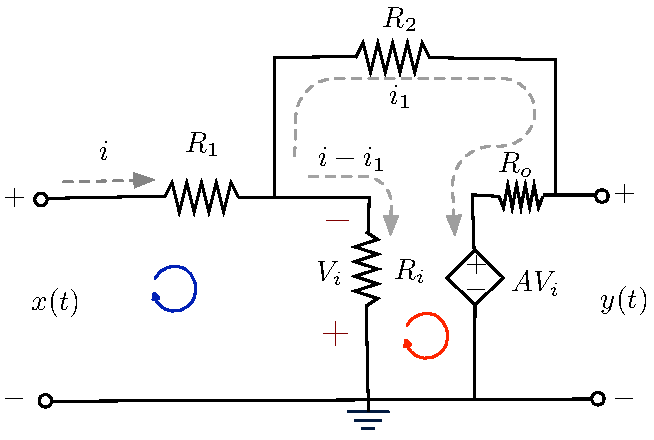
\includegraphics[width=4in]{plots/multiplierbadri3.pdf}
\captionof{figure}{The operational amplifier circuit with the model}
 \label{Fig-Prob2.1c}
}

Applying Kirchoff's law to the outer loop indicated in blue in Fig.~\ref{Fig-Prob2.1c}, we obtain the following equation.
\begin{equation}
x(t) = iR_1+(i-i_1)R_i = i(R_1+R_i) - i_1 R \label{eqn-Prob2.1.1}
\end{equation}
Note that by definition, the voltage $V_i$ that controls the VCVS is the voltage across $R_i$ measured against the indicated direction of the current $i-i_1$, and is given by
\begin{equation}
V_i = -(i-i_1)R_i. \label{eqn-Prob2.1.2}
\end{equation}
Next, writing out the Kirchoff's law for the inner loop indicated in red, we obtain the following.
\begin{align}
0 &= i_1 R_2 + i_2 R_0 + AV_i - (i-i_1) R_i
\end{align}
Substituting $V_i$ in the above equation with the RHS of \eqref{eqn-Prob2.1.2}, we obtain the following.
\begin{align}
0&= i_1 (R_2+R_0) - A(i-i_1)R_i-(i-i_1)R_i\\
&= -i(1+A)R_i+i_1((1+A)R_i+R_0+R_2)\label{eqn-Prob2.1.3}
\end{align}
Combining \eqref{eqn-Prob2.1.3} and \eqref{eqn-Prob2.1.1}, we obtain the following linear system of equations governing the electrical circuit.
\begin{align}
\left[\begin{array}{cc} R_1+R_i &  -R_i\\ -(1+A)R_i & (1+A)R_i+R_0+R_2\end{array}\right]\left[\begin{array}{c} i\\ i_1\end{array}\right] = \left[\begin{array}{c} x(t)\\ 0\end{array}\right]
\end{align}
Solving the above linear system, we identify the current in the different branches to be
\begin{align}
\left[\begin{array}{c} i\\ i_1\end{array}\right] = x(t)\left[\begin{array}{c} \frac{ (1+A)R_i+R_0+R_2}{(1+A) R_iR_1+R_0R_1+R_2R_1+R_0R_i+R_2R_i}\\ \frac{(1+A)R_i}{(1+A) R_iR_1+R_0R_1+R_2R_1+R_0R_i+R_2R_i}\end{array}\right].\label{eqn-Prob2.1.4}
\end{align}
Lastly, notice that
\begin{align}
y(t) &= i_1 R_0 + A V_i \\
 & = i_1 R_0 - (i-i_1)R_i.
\end{align}
Substituting the solutions for $i$ and $i_1$ in terms of $x(t)$, we obtain the following.
\begin{align}
y(t)= \left( \frac{R_iR_0 - R_2R_iA}{(1+A) R_iR_1+R_0R_1+R_2R_1+R_0R_i+R_2R_i} \right)x(t)
\end{align}


\end{solution}


\item \label{exer:twomassspringtwowalls} Figure~\ref{mech:twomassspringtwowalls} depicts a mechanical system involving two masses, two springs, and a damper connected between two walls.  Suppose that the spring $K_2$ is at rest when the mass $M_2$ is at position $p(t) = 0$.  A force, represented by the signal $f$, is applied to mass $M_1$.  Derive a differential equation relating the force $f$ and the position $p$ of mass $M_2$.  Determine the force $f$ in the case that the position $p(t) = e^{-t^2}$ and $M_1=M_2=\tfrac{1}{2}$ and $K_1 = K_2 = B = 1$.

\begin{solution}
Let $p_1$ be a signal representing the position of mass $M_1$.  Suppose that the spring $K_1$ connecting masses $M_1$ and $M_2$ is a rest when the masses are distance $d_1$ apart, i.e., $p - p_1 = d_1$.  The force applied by spring $K_1$ on mass $M_2$ is 
\[
f_1 = -K_1(p - p_1 - d_1) = -K_1(p - g)
\] 
where $g = p_1 + d_1$.  The force applied by spring $K_1$ on mass $M_1$ is then $-f_1$.  The force applied by the damper on $M_1$ is
\[
f_d = -BD p_1 = -BD(g - d_1) = - BD g.
\]
The total force applied to $M_1$ is $f + f_d - f_1$ and by Newton's law
\[
M_1 D^2 p_1 = M_1 D^2g = f + f_d - f_1 = f - BDg + K_1(p - g).
\]
The force applied to $M_2$ by the spring $K_2$ is
\[
f_2 = -K_2 p 
\] 
because the spring is assumed to be at rest when $p = 0$.  The total force applied to $M_2$ is $f_1 + f_2$ and by Newton's law
\[
M_2 D^2p = f_1 + f_2 =  -K_1(p - g) - K_2p.
\]
Rearranging gives
\[
K_1 g = (K_1+K_2)p + M_2 D^2p
\]
and
\[
-K_1(p - g) = M_2 D^2p  + K_2p .
\]
Now,
\[
M_1 D^2g + BDg + M_2 D^2p  + K_2p = f 
\]
and so
\[
K_1K_2 p + B(K_1+K_2)Dp + (M_1K_1 + M_1K_2 + K_1 M_2) D^2p  + BM_2D^3p + M_1M_2 D^4p = K_1 f .
\]
In the case that $M_1 = K_1 = K_2 = B = 1$ and $M_2 = 2$ we have
\[
p + 2Dp + 4D^2p + 2D^3p + 2D^4p = f.
\]
and if $p(t) = e^{-t^2}$ we have
\[
f(t) = (32 t^4-16 t^3-80 t^2+20 t+17) e^{-t^2}, \qquad g(t)=(8 t^2 - 2) e^{- t^2 }
\]
The solultion is animated in Figure~\ref{} under the assumption that $d = 2.5$.

\begin{figure}[tp]
  \centering
  \defaultanimation{tikzfigs/twomassestwowalls}
%\animategraphics[autoplay,loop,every=\every]{\defaultframerate}{}{}{}
  \caption{Motion of masses $M_1$ and $M_2$ when postition of masses $M_1$ is $p(t) = e^{-t^2}$.} \label{fig:twomassestwowallsanimanim}
\end{figure}


\end{solution}

\begin{figure}[p]
\centering
\begin{tikzpicture}
\tikzstyle{spring}=[thick,decorate,decoration={coil,pre length=0.3cm,post length=0.3cm,segment length=6,aspect=0.9}]
\tikzstyle{damper}=[thick,decoration={markings,  
  mark connection node=dmp,
  mark=at position 0.5 with 
  {
    \node (dmp) [thick,inner sep=0pt,transform shape,rotate=-90,minimum width=15pt,minimum height=3pt,draw=none] {};
    \draw [thick] ($(dmp.north east)+(2pt,0)$) -- (dmp.south east) -- (dmp.south west) -- ($(dmp.north west)+(2pt,0)$);
    \draw [thick] ($(dmp.north)+(0,-5pt)$) -- ($(dmp.north)+(0,5pt)$);
  }
}, decorate]
\tikzstyle{ground}=[fill,pattern=north east lines,draw=none,minimum width=0.75cm,minimum height=0.3cm]
\tikzstyle{wall}=[fill,pattern=north east lines,draw=none,minimum width=0.3cm,minimum height=2cm]

\node (Wleft) [wall] {};
\draw (Wleft.north east)--(Wleft.south east);

\node (M1) [minimum width=1cm,minimum height=2cm,style={draw,outer sep=0pt,thick},xshift=2.65cm] {$M_1$};
\draw [damper] (Wleft.east)--(M1.west) node[pos=0.5,above,minimum height=30pt] {$B$};
%\draw [-latex,thick] (M1.north) ++(-0.5cm,0.3cm) -- +(1cm,0) node[pos=0.5,above] {$f(t)$};
\draw [-latex,thick] (M1.south) ++(-0.5cm,-0.3cm) -- +(1cm,0) node[pos=0.5,below] {$f(t)$};

\node (M2) [minimum width=1cm,minimum height=2cm,style={draw,outer sep=0pt,thick},xshift=5.15cm] {$M_2$};
\draw [spring] (M1.east)--(M2.west) node[pos=0.5,above,minimum height=20pt] {$K_1$};
\draw [-latex,thick] (M2.south) ++(-0.5cm,-0.3cm) -- +(1cm,0) node[pos=0.5,below] {$p(t)$};

\node (Wright) [wall,xshift=7.8cm] {};
\draw (Wright.north west)--(Wright.south west);
\draw [spring] (M2.east)--(Wright.west) node[pos=0.5,above,minimum height=20pt] {$K_2$};
%\draw [thick,<->] (Wleft.north east)++(0,0.25cm) -- ++(7.5cm,0) node[pos=0.5,above] {$d$};

\end{tikzpicture}
\caption{Two masses, a spring, and a damper connected between two walls for Exercise~\ref{exer:twomassspringtwowalls}.} \label{mech:twomassspringtwowalls}
\end{figure}



\item \label{exer:dcmotorpotfeedback} Consider the electromechanical system in Figure~\ref{fig:dcmotorpotfeedback}.  A direct current motor is connected to a potentiometer in such a way that the voltage at the output of the potentiometer is equal to the angle of the motor $\theta$.  This voltage is fed back via a unity gain amplifier to the input terminal of the motor.  An input voltage $v$ is applied to the other terminal on the motor.  Find the differential equation relating $v$ and $\theta$.  What is the input voltage $v$ if the motor angle satisfies $\theta(t) = \frac{\pi}{2} (1 + \operatorname{erf}(t) )$?  Plot $\theta$ and $v$ in this case when the motor coefficients satisfy $L=0$, $R = \tfrac{3}{4}$, and $K_b=K_\tau=B=J=1$.
%Find the transfer function of the system that maps the input voltage $v$ to the motor angle $\theta$.  %Under the assumption that the motor coefficients satisfy $L=0$ and $K_b=K_\tau=B=R=J=1$ draw a pole zero plot and determine whether this system is stable and/or regular.  Find and plot the impulse response and step response if they exist.

{
\begin{figure}[tp]
  \centering
  \newcommand{\arcdegree}{25}
  \begin{circuitikz} \draw
    (4,0) to[open] (4,3) to[R, l=$R$,-o] (0,3);
    %to[short] (0,4);
    %to[short] (7.75,4) to[short,-o] (7.75,1.5);
    \draw (7,2.5) to[potentiometer,*-*] (7,0.5);
    \draw (0,-1.5) to[open, v^>=$v$,o-o] (0,3);
    \draw (5.5,-0.5) node[op amp,yscale=0.50,xscale=-0.50] {};
    \draw (7.75,1.5) to[short] (7.75,-0.75) to[short] (6,-0.75);
    \draw (5,-0.5) to[short] (4,-0.5) to[short] (4,0);
    \draw (4.75,-0.5) to[short] (4.75,0.4) to[short] (6.5,0.4) to[short] (6.5,-0.25) to[short] (6,-0.25);
    \draw (7.5,1.5) to[short,-o] (9,1.5);
    %\draw (3,-1) node[ground] {};
    \draw (0,-1.5) to[short] (9,-1.5) to[open,o-o,v>=$\theta$] (9,1.5);
    \begin{scope}[xshift=4cm,yshift=1.5cm]
      \node (M) [circle,style={draw,thick}] {motor};
      \node [right of=M, minimum width=1cm,rectangle,style={draw,thick},node distance=1.8cm] (J) {$J$};
      \draw (M.east) -- (J.west);
      \draw [->,>=stealth'] (J.east) -- +(0.4cm,0) node[] {};
      \draw [-latex] (M.west) ++(-0.2cm,-0.5cm) -- +(0cm,1.0cm) node[pos=0.5,left] {$v_b$};
      \draw (M.north) -- (0,3-1.5);
      \draw (M.south) -- (0,0-1.5);
      \begin{scope}[yshift=1cm,xshift=0.8cm]
        \draw [latex-,thick] (\arcdegree:1) arc (\arcdegree:-\arcdegree:1);
        \node at (0:1) [right] {$\theta$};
      \end{scope}
    \end{scope}
  \end{circuitikz}
  \caption{Diagram for a rotary direct current (DC) with potentiometer feedback for Exercise~\ref{exer:dcmotorpotfeedback}.} \label{fig:dcmotorpotfeedback}
\end{figure}
}

\begin{solution}
The input voltage to the DC motor is $v - \theta$.  From~(\zref{eq:dcmotordiffequation}) of the lecture notes the relationship between the input voltage and motor angle is
\[
v - \theta = \left(\frac{RB}{K_\tau} + K_b\right) D\theta + \frac{RJ}{K_\tau} D^2\theta
\] 
and so
\[
v = \theta + \left(\frac{RB}{K_\tau} + K_b\right) D\theta + \frac{RJ}{K_\tau} D^2\theta.
\]
If $\theta(t) = \frac{\pi}{2} (1 + \operatorname{erf}(t) )$ then
\[
D\theta(t) = \sqrt{\pi} e^{-t^2}, \qquad D^2\theta(t) = -2t \sqrt{\pi} e^{-t^2}
\]
and so
\[
v(t) = {{\pi\,\left(\mathrm{erf}\left(t\right)+1\right)}\over{2}}-2\,
 \sqrt{\pi}\,t\,e^ {- t^2 }+2\,\sqrt{\pi}\,e^ {- t^2 }
\]
The signals $v$ and $\theta$ are plotted in the figure below.  Observe that as $t \to \infty$ both $\theta(t)$ and $v(t)$ converge to $\pi$.

\begin{figure}[tp]
  \centering
  \defaultanimation{tikzfigs/dcmotorstabilised}
%\animategraphics[autoplay,loop,every=\every]{\defaultframerate}{}{}{}
  \caption{Voltage and corresponding angle for the dc motor with potentiometer in Figure~\ref{fig:dcmotorpotfeedback} with constants $L =0$, $R = \tfrac{3}{4}$, and$K_b=K_\tau=B=J=1$.} \label{fig:dcmotorpotfeedbackdcmotoranim}
\end{figure}


% The transfer function is
% \[
% \frac{\calL(v)}{\calL(\theta)} = \frac{1}{1 + \left(\frac{RB}{K_\tau} + K_b\right) s  + \frac{RJ}{K_\tau} s^2}.
% \]
% Under the assumption that $K_b=K_\tau=B=R=J=1$ the transfer function is
% \[
% \frac{\calL(v)}{\calL(\theta)} = \frac{1}{1 + 2s  + s^2} = \frac{1}{(1 + s)^2}.
% \]
% There are two equal real poles at $s = -1$ and no zeros.  A pole zero plot is below.

% \begin{center}
%   \begin{tikzpicture}
%     \poletikz{-1}{0} \node[below] at (-1,0) {$-1$};
%     \polezeroaxis{2}
%   \end{tikzpicture}
% \end{center}

% The system is regular because there are more poles than zeros.  The system is stable because there are at least as many poles as zeros and all poles have negative real part.  The impulse response is found to be $h(t) u(t) t e^{-t}$ by application of the inverse Laplace transform.  The step response is given by application of the integrator system
% \[ 
% H(u) = I_\infty(h) = \int_{-\infty}^t u(\tau) t e^{-\tau} d\tau = \int_{0}^t t e^{-\tau} d\tau = u(t) \big( 1 - e^{-t}(t+1) \big).
% \] 
% These responses are plotted below

% \begin{center}
% \begin{tikzpicture}
% \begin{scope}[yscale=4]
%     \draw[->] (-1,0) -- (10,0) node[above] {$t$};
%     \draw[->] (0,-0.1) -- (0,0.5) node[right] {$u(t) t e^{-t}$};
%     \draw[thick] (-0.5,0) -- (0,0) {};
%     \draw[color=black,thick] plot[domain=0:9,samples=101,smooth] function{x*exp(-x)};
%     \htick{0.3} node[pos=0.5,left] {$0.3$};
% \end{scope}
%     \vtick{1} node[pos=0.5,below] {$1$};
%     \vtick{7} node[pos=0.5,below] {$7$};
% \end{tikzpicture}

% \begin{tikzpicture}
% \begin{scope}[yscale=2]
%     \draw[->] (-1,0) -- (10,0) node[above] {$t$};
%     \draw[->] (0,-0.2) -- (0,1.3) node[right] {$u(t) \big( 1 - e^{-t}(t+1) \big)$};
%     \draw[thick] (-0.5,0) -- (0,0) {};
%     \draw[color=black,thick] plot[domain=0:9,samples=101,smooth] function{1-(x+1)*exp(-x)};
%     \htick{1} node[pos=0.5,left] {$1$};
% \end{scope}
%     \vtick{1} node[pos=0.5,below] {$1$};
%     \vtick{7} node[pos=0.5,below] {$7$};
% \end{tikzpicture}
% \end{center}


\end{solution}


\end{excersizelist}


%%% Local Variables: 
%%% mode: latex
%%% TeX-master: "main.tex"
%%% End: 
